\section{Fused MoE Kernel Design}\label{sec:method}
\begin{figure}[!ht]
    \centering
    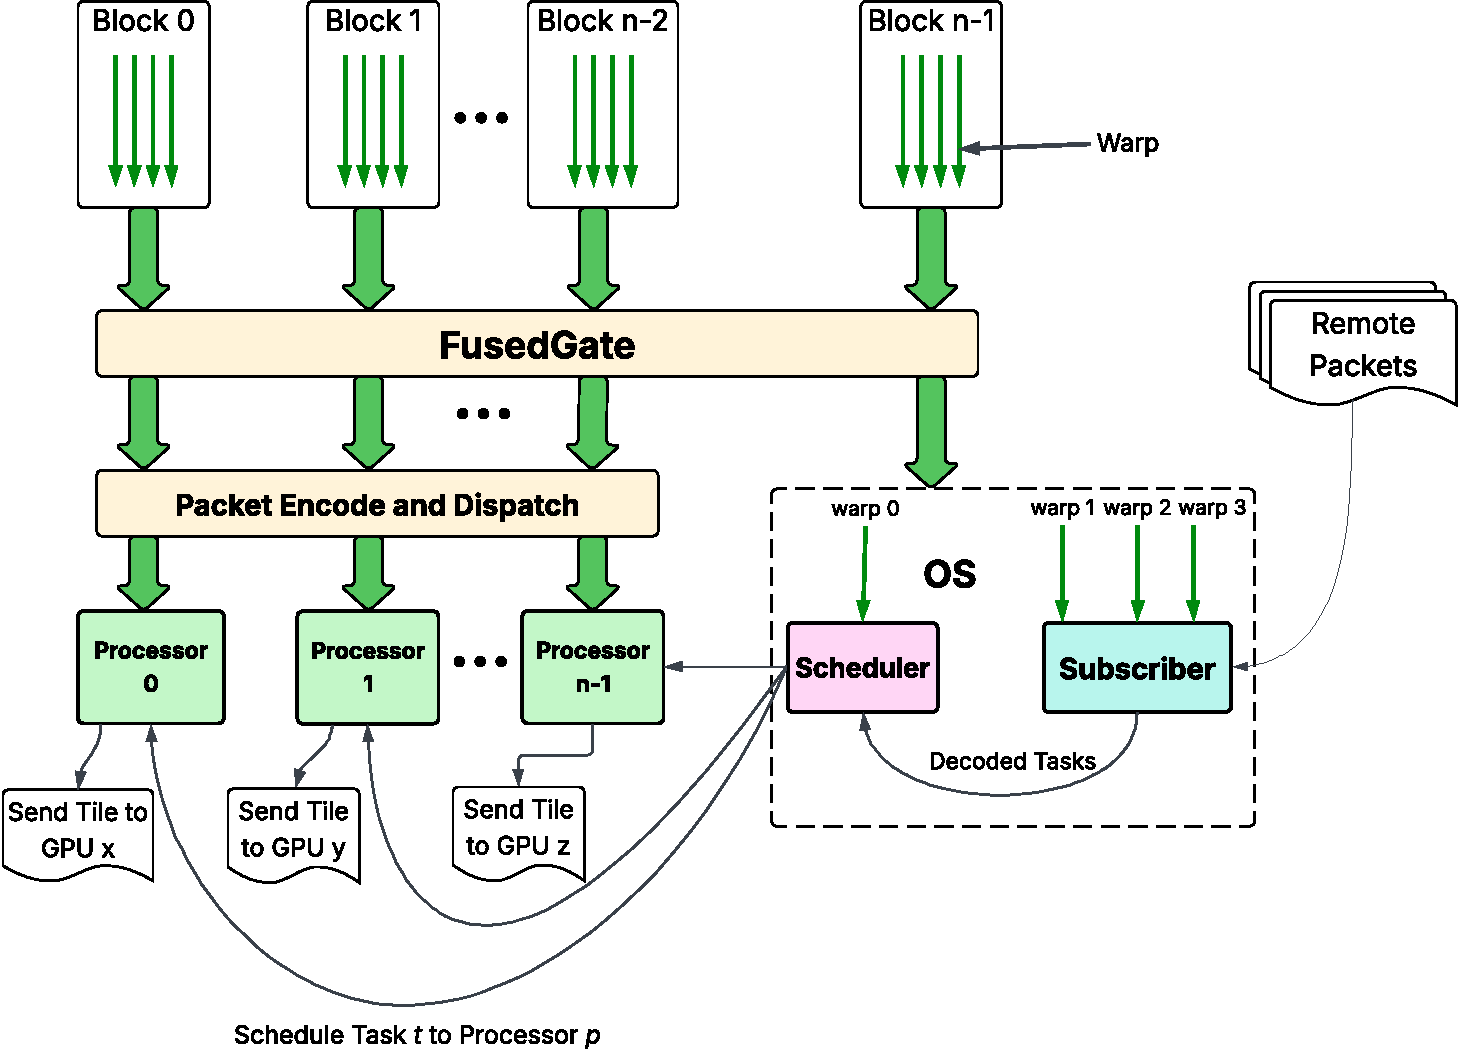
\includegraphics[width=0.8\textwidth, keepaspectratio]{figures/architecture}
    \caption{\emph{\sysname Fused Kernel}}
    \label{fig:fusedK}
\end{figure}
Modern distributed MoE systems suffer from two limitations: (1) frequent many-to-many
(\emph{AlltoAll or AllGather}) collectives on the critical path, and
(2) significant overhead from repeated kernel launches.
We address these in \sysname, a fully fused MoE operator implemented
as a single persistent GPU kernel.
Unlike previous approaches~\cite{comet, deepep, pmlr-v162-rajbhandari22a, megatron, MLSYS2023_5616d34c,
    MLSYS2024_339caf45, 10.1145/3503221.3508418, 10.1145/3588964, 10.1145/3627703.3650083, 10.1145/3710848.3710868,
    NEURIPS2022_67d57c32},
\sysname is the first solution to implement a \emph{completely fused Distributed MoE kernel},
eliminating kernel launch overhead entirely by requiring only a single kernel launch (see Table~\ref{tab:gpuOps}).
\SetKwInput{KwRequire}{Require}
\SetKwInput{KwResult}{Result}
\SetKwInput{KwInput}{Input}
\SetKw{kwAnd}{and}
\SetKw{kwOr}{or}
\SetKw{kwTrue}{True}
\SetKw{kwFalse}{False}
\begin{algorithm}[!h]
    \small
    \DontPrintSemicolon
    \caption{~\emph{\sysname Distributed MoE Fused Kernel}}\label{alg:one}
    \KwInput{$A, O \in \mathbb{R}^{S\times H},\; X \in \mathbb{R}^{E\times H \times D},\; N$}
    \Begin{
        $T_{\phi}, G_{\phi} \gets \mathbf{FusedGate}(A)$\;
        \eIf{$\text{blockId} + 1 < N$}{
            $\mathbf{Dispatch}(T_{\phi}, A)$\;
            processor::start()\;
        }{
            \eIf{$warpID == 0$}{
                scheduler::start()\;
            }{
                subscriber::start($T_{\phi}$, $G_{\phi}$, $O$, $X$)\;
            }
        }
    }
\end{algorithm}
\begin{figure}[!ht]
    \centering
    \vspace{-3mm}
    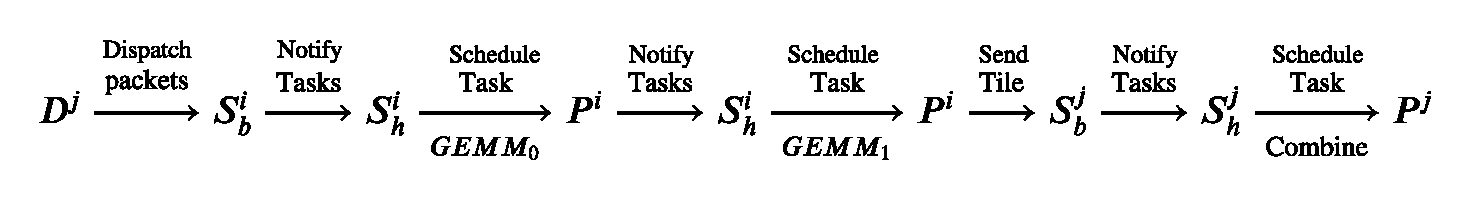
\includegraphics[width=\linewidth]{figures/actors}
    \caption{\emph{DMoE Functional Dependencies Expressed as a Chain of Actor Interactions}.
    We denote $S_b$, $S_h$, and $P$ as the
    Subscriber, Scheduler and Processor actors, respectively. For any actor $a \in \{S_b,\>S_b,\>P\}$,
        $a^i$ identifies an actor on GPU $i$. We define $D^j_i$ as the operator,
        where GPU $j$ dispatches packets of tiles to GPU $i$,
        This diagram expresses task dependencies at the granularity of a tile, namely
        $GEMM_0$, $GEMM_1$, combine and communication produce an output tile.
        Notifications occur as signals propagated through shared memory (subscriber $\leftrightarrow$ scheduler) or
        global memory (scheduler $\leftrightarrow$ processor or inter-GPU communication). Note one-sided
        inter-GPU transfers (packet or single tile) are \emph{coupled} with a signal to
        notify $S_b^j$ on the receiving GPU $j$ of the message's delivery.
    }
    \label{fig:actors}
    \vspace{-4mm}
\end{figure}

\myparab{Actor-based model.}
The design of \sysname is based on the actor model of concurrent
computation~\cite{agha:85, 10.5555/1624775.1624804, Greif:75}.
We implement this model by specializing GPU thread blocks and warps into three distinct actor roles:
(1) \textbf{Processor} (\S\ref{subsec:processor}), (2) \textbf{Subscriber} (\S\ref{subsec:subscriber}),
and (3) \textbf{Scheduler}(\S\ref{subsec:scheduler}).
The Processor performs compute (GEMMs and element-wise operations) and tile communication.
We use CUTLASS~\cite{Thakkar_CUTLASS_2023} as the underlying infrastructure for high-performance
BLAS routines and NVSHMEM for kernel-initiated communication~\cite{nvshm}.
The Subscriber and Scheduler perform administrative functions.
Specifically, the Scheduler assigns computational tasks to available thread blocks.
Our key innovation is making the Scheduler both \emph{multithreaded},
enabling high scheduling throughput, and \emph{work-conserving}, ensuring consistently high GPU SM utilization.
On the other hand, the Subscriber decodes \emph{tile packets} from peer GPUs to task descriptors
(\S\ref{subsec:task-abstraction-for-computation}).
Of the $N$ thread blocks on a GPU, we specialize $N-1$ to adopt the \textbf{Processor} role.
We specialize the last block as the Operating System (OS).
Within this block, we specialize three warps for the \textbf{Subscriber} role and
one warp for the \textbf{Scheduler} role.
This split of thread blocks across actors is intentional: our goal is to use few resources for administrative
tasks while reserving bulk of the resources for performing MoE computation tasks.
Figure~\ref{fig:fusedK} summarizes the
\sysname architecture and its constituent actors, while Algorithm~\ref{alg:one} gives a very close translation of the
system in code.
Note that $A \in \mathbb{R}^{S \times H}$ is the input token matrix;
$O \in \mathbb{R}^{S \times H}$ the output matrix;
and $X \in \mathbb{R}^{E\times H \times D}$ is a 3-D tensor of expert weights,
where $E$ denotes the number of local experts for the executing GPU, $H$ is the embedding dimension,
$D$ is the FFN intermediate dimension and $S$ is the sequence length.
$T_{\phi} \in \left(\mathbb{R}^2\right)^{E \times C}$
is a routing table data structure, where $T_{\phi}\left( e, c\right) = (i, w)$ indicates that token $i$ at slot $c$
dispatches to expert $e$. $w$ is the combine weight (Equation~\ref{eq:combine1}) and $C$ is expert capacity.
The tuple structure of $T_{\phi}$ is an implementation detail. $G_{\phi} \in \mathbb{R}^{S \times E}$ captures
the affinity scores produced by the gate (Equation~\ref{eq:combine2}).

\begin{figure}[!ht]
    \centering
    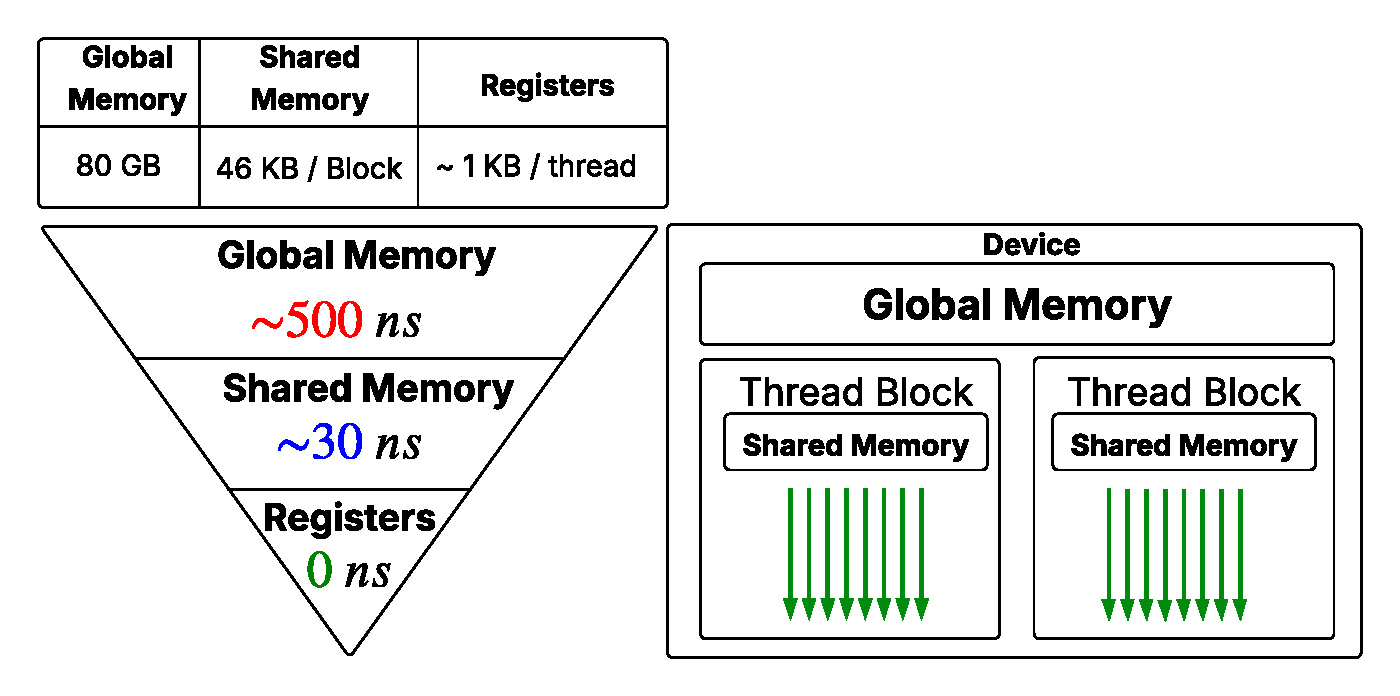
\includegraphics[width=3.5in]{figures/mem2}
    \caption{\emph{GPU Memory Hierarchy}.
    The inverted pyramid (left) shows the load/store access latency~\cite{10579250, amperearch, ptx}.
    The table above outlines the capacity for different memory tiers (for A100 GPUs).
    The shared memory and register capacity are static configurations for \sysname.
    The right figure shows accessibility scopes: on-chip \textbf{registers}
    are scoped to a thread; on-chip \textbf{shared memory} is visible to all threads in a block;
    and off-chip \textbf{global memory} is accessible by all threads on device.}
    \label{fig:mem}
    \vspace{-3mm}
\end{figure}

\myparab{Inter-actor interactions in \sysname.}
\sysname decomposes MoE computation and communication at the granularity of a tile, a statically sized partition of a tensor,
to achieve parallel execution and efficient overlap of tasks.
Each tile maps to a discrete unit of work encapsulated by a \emph{task descriptor}.
The \textbf{Subscriber} decodes these task descriptors from the remote tile packets it receives.
Concurrently, the \textbf{Scheduler} receives notifications about available tasks and dispatches them for execution
to \textbf{Processor} actors that perform computations defined by these tasks,
namely the feed-forward network (FFN) and expert-combine operations.
Figure~\ref{fig:actors} show the chain of actor interactions, demonstrating how \sysname
enforces DMoE functional dependencies.

\myparab{Determining tile dimensions in \sysname.}
Selecting appropriate tile dimensions in \sysname is crucial to ensure efficient GPU utilization.
An undersized tile underutilizes the GPU,
while excessively large tiles create register pressure,
causing performance-degrading register spills to local memory.
After careful parameter sweeps,
we choose tile dimensions of (128, 64).
Our key insights are: increasing tile width significantly raises the register usage per thread,
potentially triggering costly spills;
increasing tile height without adjusting thread count increases workload per thread, harming performance.
Raising the thread count per block beyond our fixed value of 128 threads reduces the number of concurrent blocks,
negatively affecting SM occupancy.
Larger thread-block sizes also increase overhead from intra-block synchronization (\emph{\_\_syncthreads()} barriers),
further degrading performance.
Thus, our chosen tile dimensions balance register usage, shared-memory constraints,
and GPU occupancy to deliver optimal performance.

\subsection{Task Abstraction for Computation}\label{subsec:task-abstraction-for-computation}

\myparab{Computational operators.}
The FFN operator is a standard position-wise feed-forward network widely used in Transformer architectures~\cite{NIPS2017_3f5ee243}, composed of two linear transformations separated by a nonlinear activation $\phi$ (e.g., GELU or ReLU):

\begin{equation}\label{eq:ffn}
    \small
\textrm{FFN}(x) = W_2 \cdot \phi(x W_1 + b_1) + b_2
\end{equation}

Here, $W_1$ and $W_2$ represent learnable weight matrices, and $b_1$ and $b_2$ are biases.
The expert-combine operation, used in architectures like GShard~\cite{DBLP:conf/iclr/LepikhinLXCFHKS21} and DeepSeek~\cite{deepep}, merges outputs from multiple experts by computing a weighted combination based on their affinity scores:
\begin{equation}\label{eq:combine1}\small
\mathcal{C}_i = \sum\limits_{j = 1}^k g_{i, e}
\end{equation}
\begin{equation}\label{eq:combine2}\small
\mathbf{h}_i = \sum\limits_{j = 1}^k \frac{g_{i, e}}{\mathcal{C}_i}\cdot \mathbf{h}_i^k
\end{equation}

In these equations, $i \in {0, S - 1}$ represents an input token index, $e = E_{i,k}$ identifies the $k$-th expert selected for token $i$, and $g_{i,e}$ is the affinity score indicating how relevant expert $e$ is for token $i$.

\myparab{Unified task abstraction.}
We unify the FFN and combine operations under a common abstraction called a \emph{task}. Tasks provide a uniform interface for communicating tile-level work among Subscribers, Schedulers, and Processors. Formally, a task descriptor $t \in \mathcal{T}$ is defined as a tuple:
\[\small
    t = (\mathcal{M}, \star, \phi)
\]

where $\mathcal{M}$ is a set of metadata (\eg  device ID, tile index), $\star$ is a binary tensor operation (specifically, matrix multiplication $\cdot$ or Hadamard product $\odot$), and $\phi$ is an element-wise activation function (e.g., ReLU or identity). 

We define a task $t$ operating on input tensors $A$, $B$, $D$, producing output tensor $C$, as follows:
\begin{equation}\label{eq:task_def}\small
    \mathcal{F}_t(A, B, C, D) \coloneqq C \gets \phi\left(A \star_t B + D\right)
\end{equation}

The operator $\star_t$ (instantiated from $\star$) may behave differently depending on the task metadata $\mathcal{M}$, and the result of $A \star_t B$ is accumulated into $D$. We provide an example of task metadata in~\S\ref{sec:task-implementation}.

In practice, we implement each task defined by Equation~\ref{eq:task_def} as a \emph{single fused} \verb|__device__|
decorated function which the \textbf{Processor} (Algorithm \ref{alg:processor}) invokes at runtime.
Fusion for $t$ entails applying $\phi$ and the succeeding addition operation to registers
storing the results of the binary operator $\star_t$.
To illustrate its flexibility, we show how the FFN and expert-combine operations can be expressed
using this task framework.
Note that we omit the matrix multiplication symbol ($\cdot$) for simplicity.
Also, $\phi_1$ can be any activation function, while $\phi_2$ is the identity function.
The FFN is expressed as:
\begin{gather*}\small
    t_1 = (\mathcal{M}, \cdot, \phi_1), \quad t_2 = (\mathcal{M}, \cdot, \phi_2), \\ \small
    \mathcal{F}_{t_1}(A, B_1, C_1, D_1) \coloneqq C_1 \gets \phi_1\left(A B_1 + D_1\right), \\ \small
    \mathcal{F}_{t_2}(C_1, B_2, C_2, D_2) \coloneqq C_2 \gets \phi_2\left(C_1 B_2 + D_2\right).
\end{gather*}
Whereas, the expert-combine operation is formalized as:
\begin{gather*}\small
    t_3 = (\mathcal{M}, \odot, \phi_2), \\ \small
    \mathcal{F}_{t_3}(A, S, C, C) \coloneqq C \gets \phi_2\left(A \odot S + C\right).
\end{gather*}
\subsection{Symmetric Tensor Layout for Inter-GPU Communication}\label{subsec:symmetric-tensor-layout}
\begin{figure}[!ht]
    \centering
    \begin{subfigure}{0.62\textwidth}
        \centering
        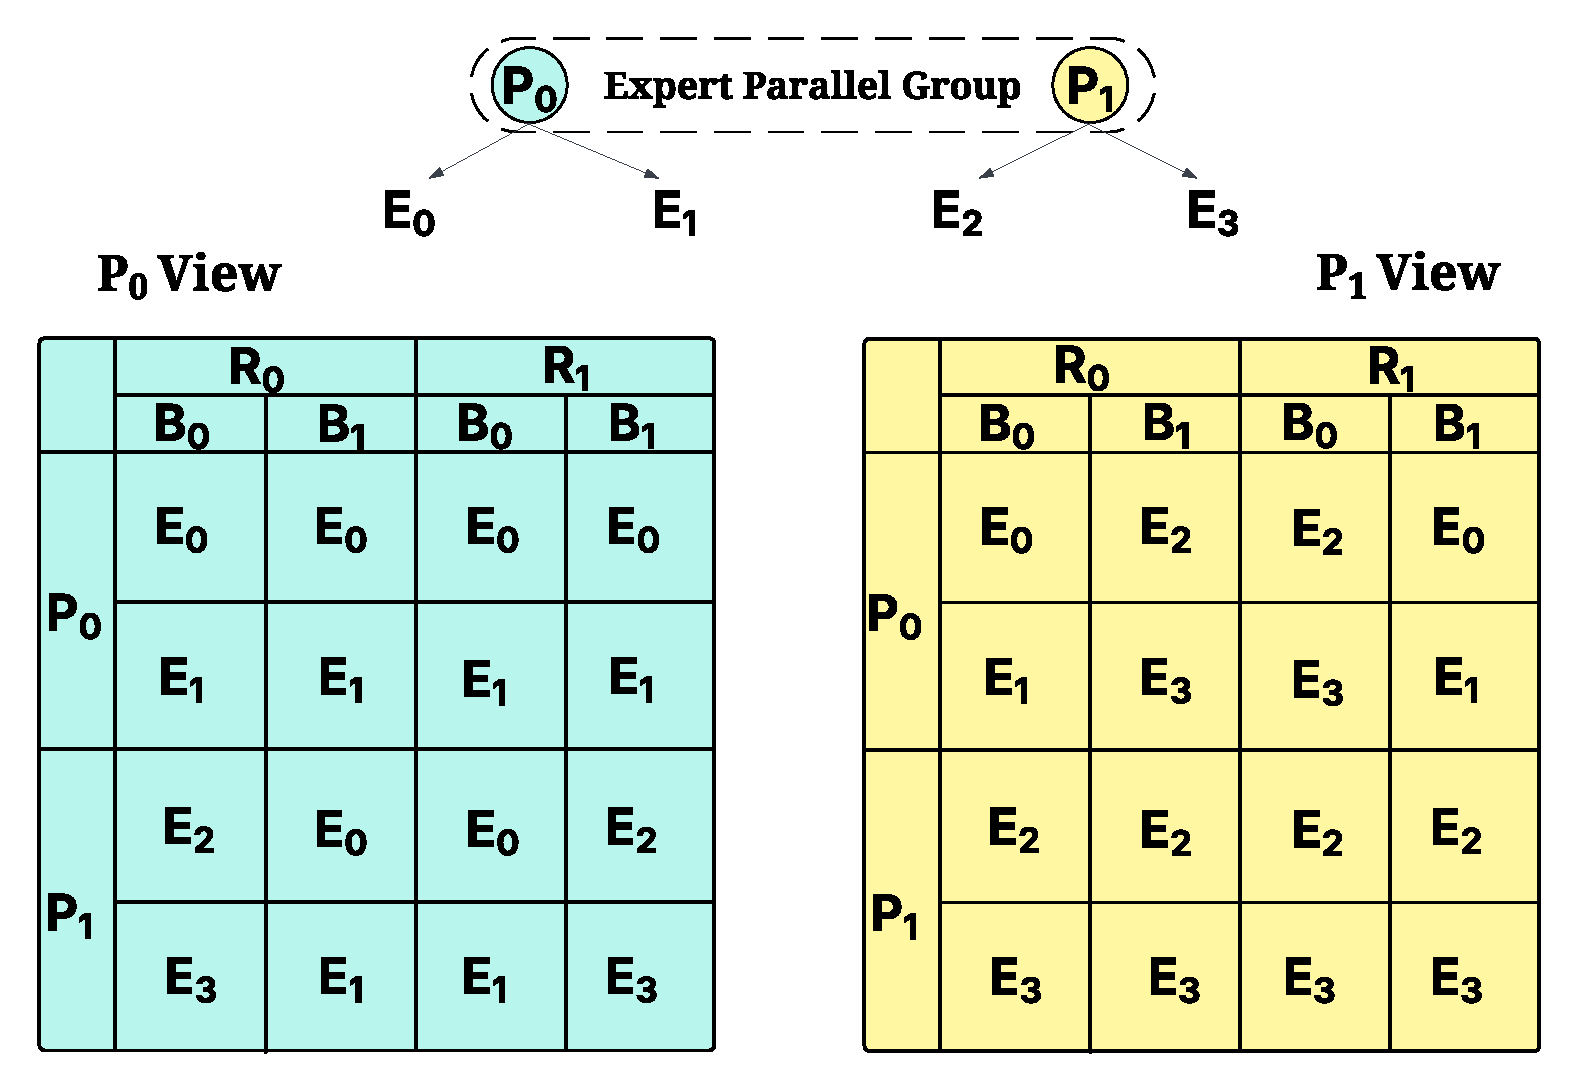
\includegraphics[width=\linewidth, keepaspectratio]{figures/mem_layout}
        \caption{\emph{Symmetric Tensor Layout across 2 Expert-parallel Processes}.}
        \label{fig:mem_layout}
    \end{subfigure}
    \begin{subfigure}{0.36\textwidth}
        \centering
        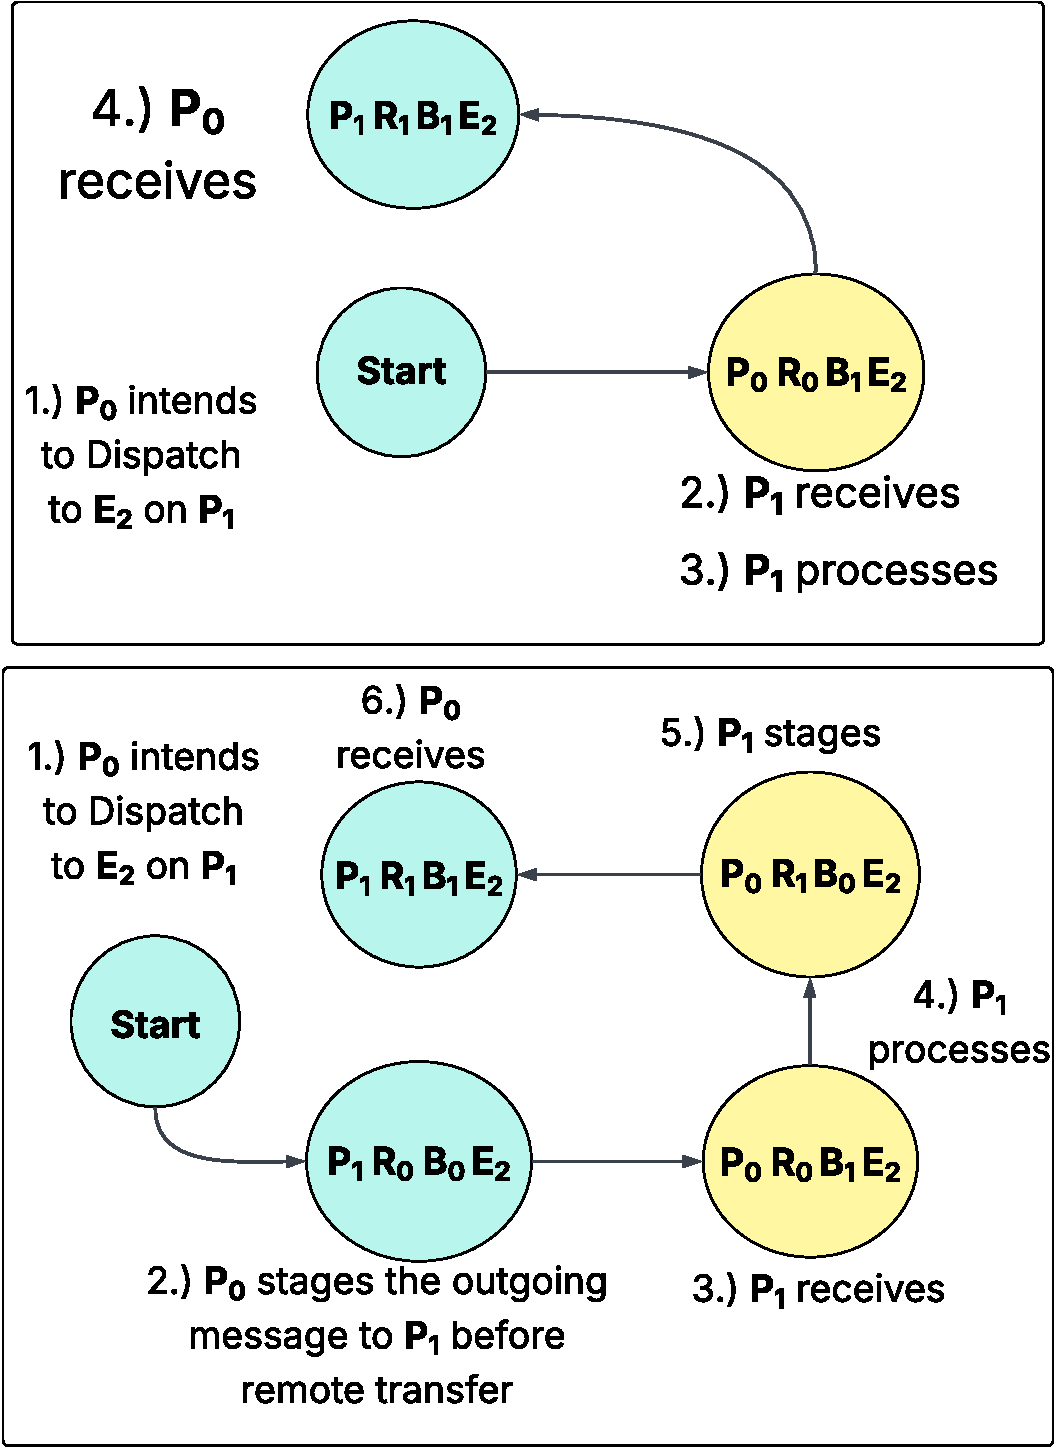
\includegraphics[width=\linewidth, keepaspectratio]{figures/sm_big}
        \caption{\emph{State machine for DMA (top) and RDMA (bottom) communication.}}
        \label{fig:sm}
    \end{subfigure}
\end{figure}

Within a single GPU device, the actors in \sysname communicate through the GPU's memory subsystem (see Figure~\ref{fig:mem}).
Specifically, the Scheduler and Subscriber actors exchange data via fast shared memory, while other actor pairs
communicate through global memory.
For communication across multiple devices, \sysname uses \emph{device-initiated communication},
leveraging the one-sided PGAS (Partitioned Global Address Space) programming model~\cite{10.1145/1278177.1278183}.
However, achieving scalable and correct one-sided memory accesses in PGAS without costly synchronization
is a known challenge~\cite{deepep, triton-dist}.
We address this challenge with a provably correct and scalable solution: a symmetric tensor layout $L$,
supporting fully non-blocking memory accesses.
We define L as:\\
\[
    L \in \mathbb{R}^{P\times R \times B \times E \times C \times H}
\]
where: $P$ is the expert parallel world size, $R$ identifies communication rounds (\ie two rounds,
one for token dispatch and one for combine), $B$ is number of staging buffers,
$E$ is the number of local experts, $C$ is the upscaled expert capacity (\S\ref{subsubsec:payload})
and $H$ is the token embedding dimension.
Our core insight to enable non-blocking communication is \emph{temporal buffering}.
Specifically, we overprovision memory for the underlying token matrix by at least $2 \cdot r$ times, where $r$
is the number of communication rounds in the dependency graph, and the factor of $2$ accounts for
separate buffers for incoming and outgoing data within each communication round.
For MoE models, we have $2 \cdot r = 4$.
This modest increase in memory usage eliminates the need for synchronization during one-sided data transfers.
Figure~\ref{fig:sm} illustrates how cells within this symmetric tensor layout are indexed
and used for Direct Memory Access (DMA) and Remote DMA (RDMA) operations.
As Theorem~\ref{theorem:ww} reinforces,
this indexing scheme over $L$ is the underlying mechanism that allows for fully non-blocking accesses eliding
synchronization because all accesses are write \emph{conflict-free}.
See\S~\ref{sec:proof-of-theorem} for the proof.
\begin{theorem}\label{theorem:ww}
   The symmetric tensor layout $L$ is write-write conflict-free.
\end{theorem}
To construct $L$, we start from the original token buffer $T \in \mathbb{R}^{S \times H}$, where $S$ is the
sequence length and $H$ is the token embedding dimension.
We first reorganize the sequence dimension $S$ into three sub-dimensions representing the expert capacity ($C$),
local expert slots ($E$), and the expert parallel world size ($W$), st:
\[
C \cdot E \cdot W = C \cdot E' = S', \quad\text{where}\quad S' \geq S \text{ and } E' \geq E_W
\]
In the typical case of uniform expert distribution (illustrated in Figure~\ref{fig:mem_layout}),
we have $S' = S$ and $E' = E_W$, where $E_W$ is the total number of experts in the model.
Thus, the size of the token buffer is $Size(T) = S' \cdot H$.
In Figure~\ref{fig:mem_layout}, each cell labeled $E_i$ (with $i \in \{0,\ldots,3\}$) is a matrix of size $(C, H)$.
Extending prior work~\cite{DBLP:conf/iclr/LepikhinLXCFHKS21, comet}, we introduce additional temporal dimensions
$R$ (communication rounds) and $B$ (staging buffers).
Each communication round has two fixed staging slots: one for outgoing tokens and another for incoming tokens.
Each slot, indexed by dimension $P$, forms a tensor of shape $(S', H)$.
Therefore, the tensor size $Size(L)$ is generally at least four times the original token buffer size,
becoming exactly four times larger in the case of uniform expert distribution. Empirically, we find:
\[
    Size(L) \approx 4 \cdot Size(T)
\]

\subsubsection{In-place Padding for Payload Efficiency}\label{subsubsec:payload}
Due to the dynamic and uneven distribution of tokens in MoE dispatch~\cite{bmamba}, GPUs commonly
receive fewer tokens than their predefined expert capacity.
Current MoE frameworks~\cite{pmlr-v162-rajbhandari22a} typically pad these buffers with null tokens before computation,
unnecessarily increasing communication payloads and degrading performance.
In contrast, we propose \emph{in-place padding}, performing padding directly within the local
symmetric tensor buffers and thus eliminating excess network communication.

As we show in Figure~\ref{fig:mem_layout} as a reference, each cell $E_i$ is sized according to the expert capacity $C$.
We further align this capacity to ensure divisibility by the tile block size $bM = 128$,
guaranteeing safe and aligned memory reads by Processor threads consuming remote tokens.
This in-place padding strategy slightly increases the memory footprint of $L$, as described below:
\[
    Size(L) \approx \begin{cases}
        4 \cdot Size(T), & \frac{S}{E} \geq bM \\[1ex]
        4 \cdot \frac{bM \cdot E}{S} \cdot Size(T), & \text{otherwise}
    \end{cases}
\]
